\section{Results} \label{Results-and-discussion}
\subsection{Transition Scenarios}
Notes for Ansh: electricity diverted to storage could be reduced to text with percentages i.e. "total amount of electricity diverted to storage=, electricity for storage came from nuclear (50\%), solar(30\%),wind(20\%) over 2017-2100". Same for H2 (total GWh generated, amount).

Scenario 1 results (fig. \ref{scen1}) demonstrate our model's attempt at decarbonization using existing technologies without deploying new nuclear power. Under these conditions, coal and oil must be retired by 2030, and natural gas by 2050. All existing nuclear power plants must restarted by <YEAR> at full operating capacity. With renewable energy as the only option for decarbonization, significant investments in solar, onshore wind, offshore wind (both fixed-bottom and floating), and lithium ion storage are necessary. The presence of a large share of renewables results in significant overgeneration of electricity during some years. Due to reduced flexibility caused by the retirement of natural gas and an increase in the share of renewables, nuclear power plants must be able to load follow, which is simulated in our model. The plot displaying the electricity supplied to the end-user shows a high degree of variability as excess electricity from renewables, hydropower, and nuclear power is often diverted to lithium-ion storage as appropriate, instead of being directly supplied to the \gls{TIMES} process. Despite the deployment of a large amount of renewables, the model fails to achieve the 2030 and 2050 emission reduction goals by <AMT1> and <AMT2> respectively. Furthermore, emissions continue to rise after 2050 primarily due to life-cycle emissions of lithium-ion batteries. The total cost of this transition is \textbf{insert number here.}


With the option of deploying new nuclear reactors available in Scenario 2 (fig. \ref{scen2}) , the model chooses to rapidly deploy nuclear power plants at the maximum allowed growth rate despite the high investment cost of nuclear, due to its low life-cycle emissions. Coal and oil are again retired rapidly, but due to the reduction in emissions by nuclear power, natural gas power plants can continue to operate. The amount of renewables required for decarbonization is reduced dramatically. This combined with the load following capabilities of natural gas plants and nuclear reactors drastically reduces the amount of lithium ion storage. The model is able to achieve its 2030 and 2050 decarbonization goals, and automatically decarbonizes more than the required limit by 2100. The total transition cost is \textbf{insert number here.}
\begin{figure}[h] 
\centering
\label{scen1}
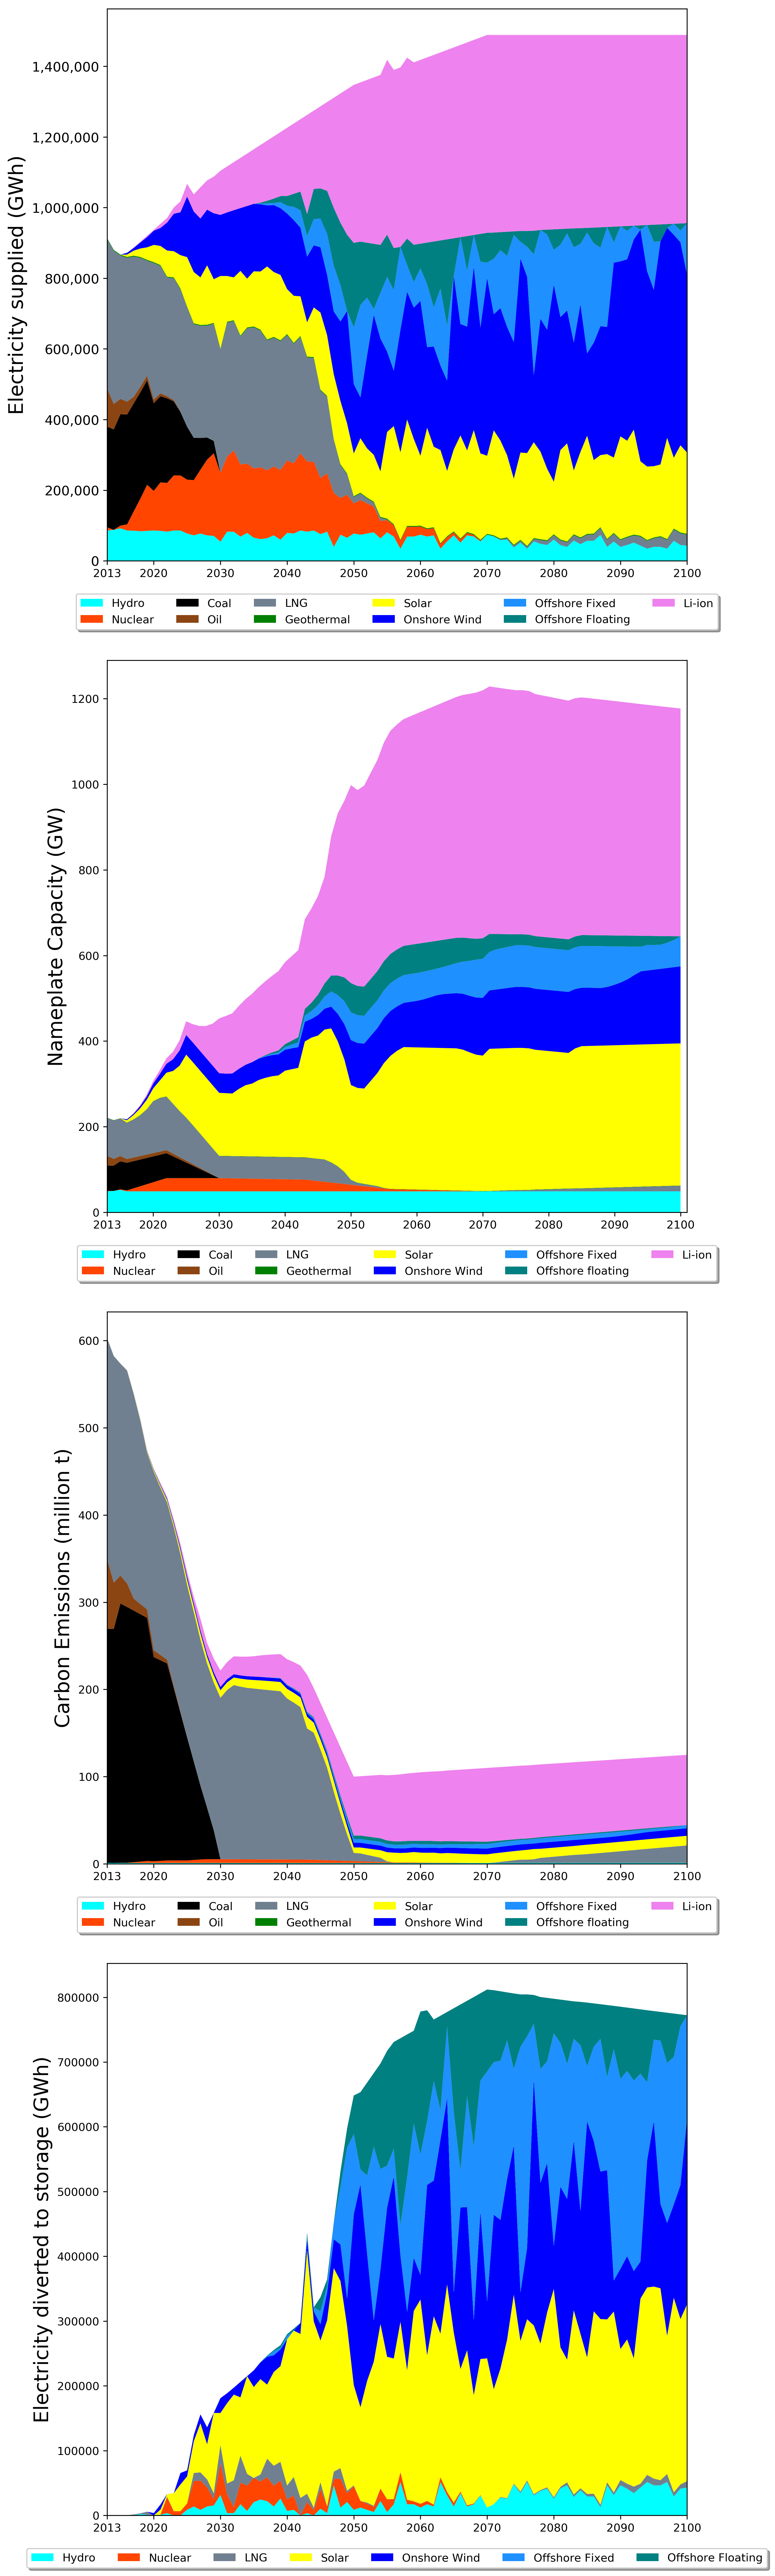
\includegraphics[scale=0.25]{figures/conv_nonuc}
\caption{Conventional technologies, no new nuclear.}
\end{figure}

\begin{figure}[h] 
\centering
\label{scen2}
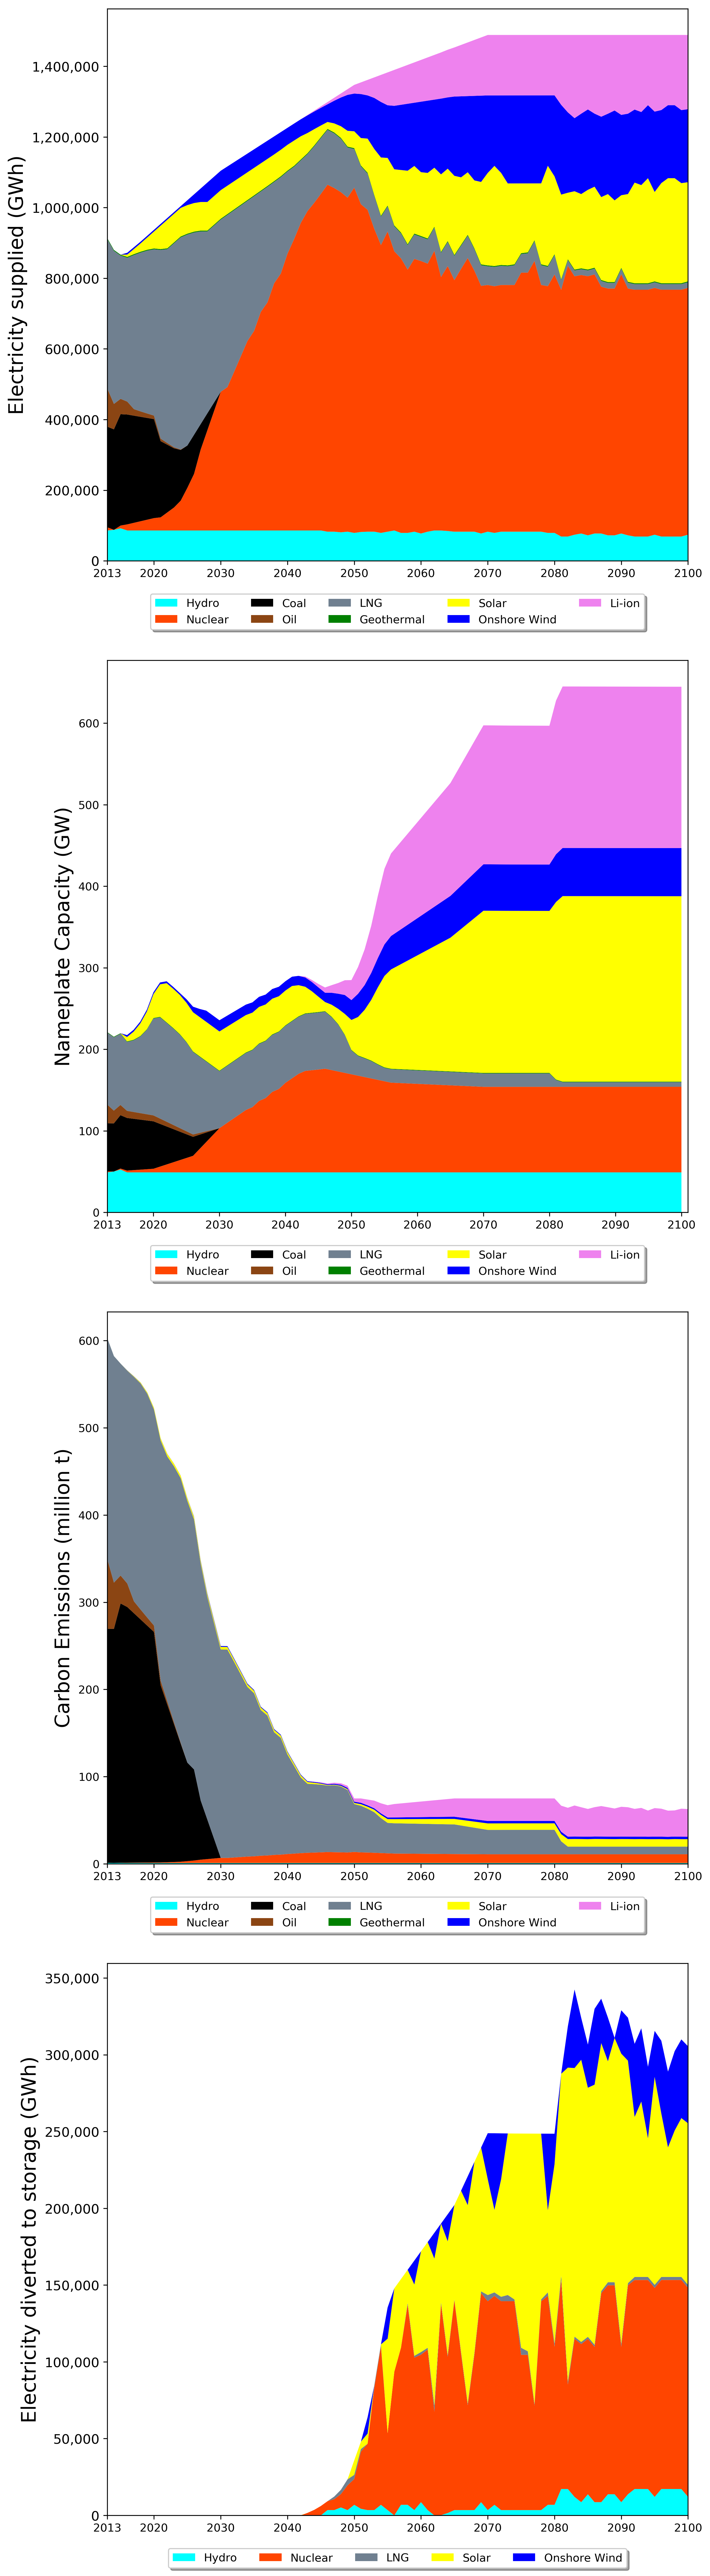
\includegraphics[scale=0.25]{figures/conv_nuc}
\caption{Conventional technologies, with new nuclear.}
\end{figure}

\begin{figure}[h] 
\centering
\label{scen3}
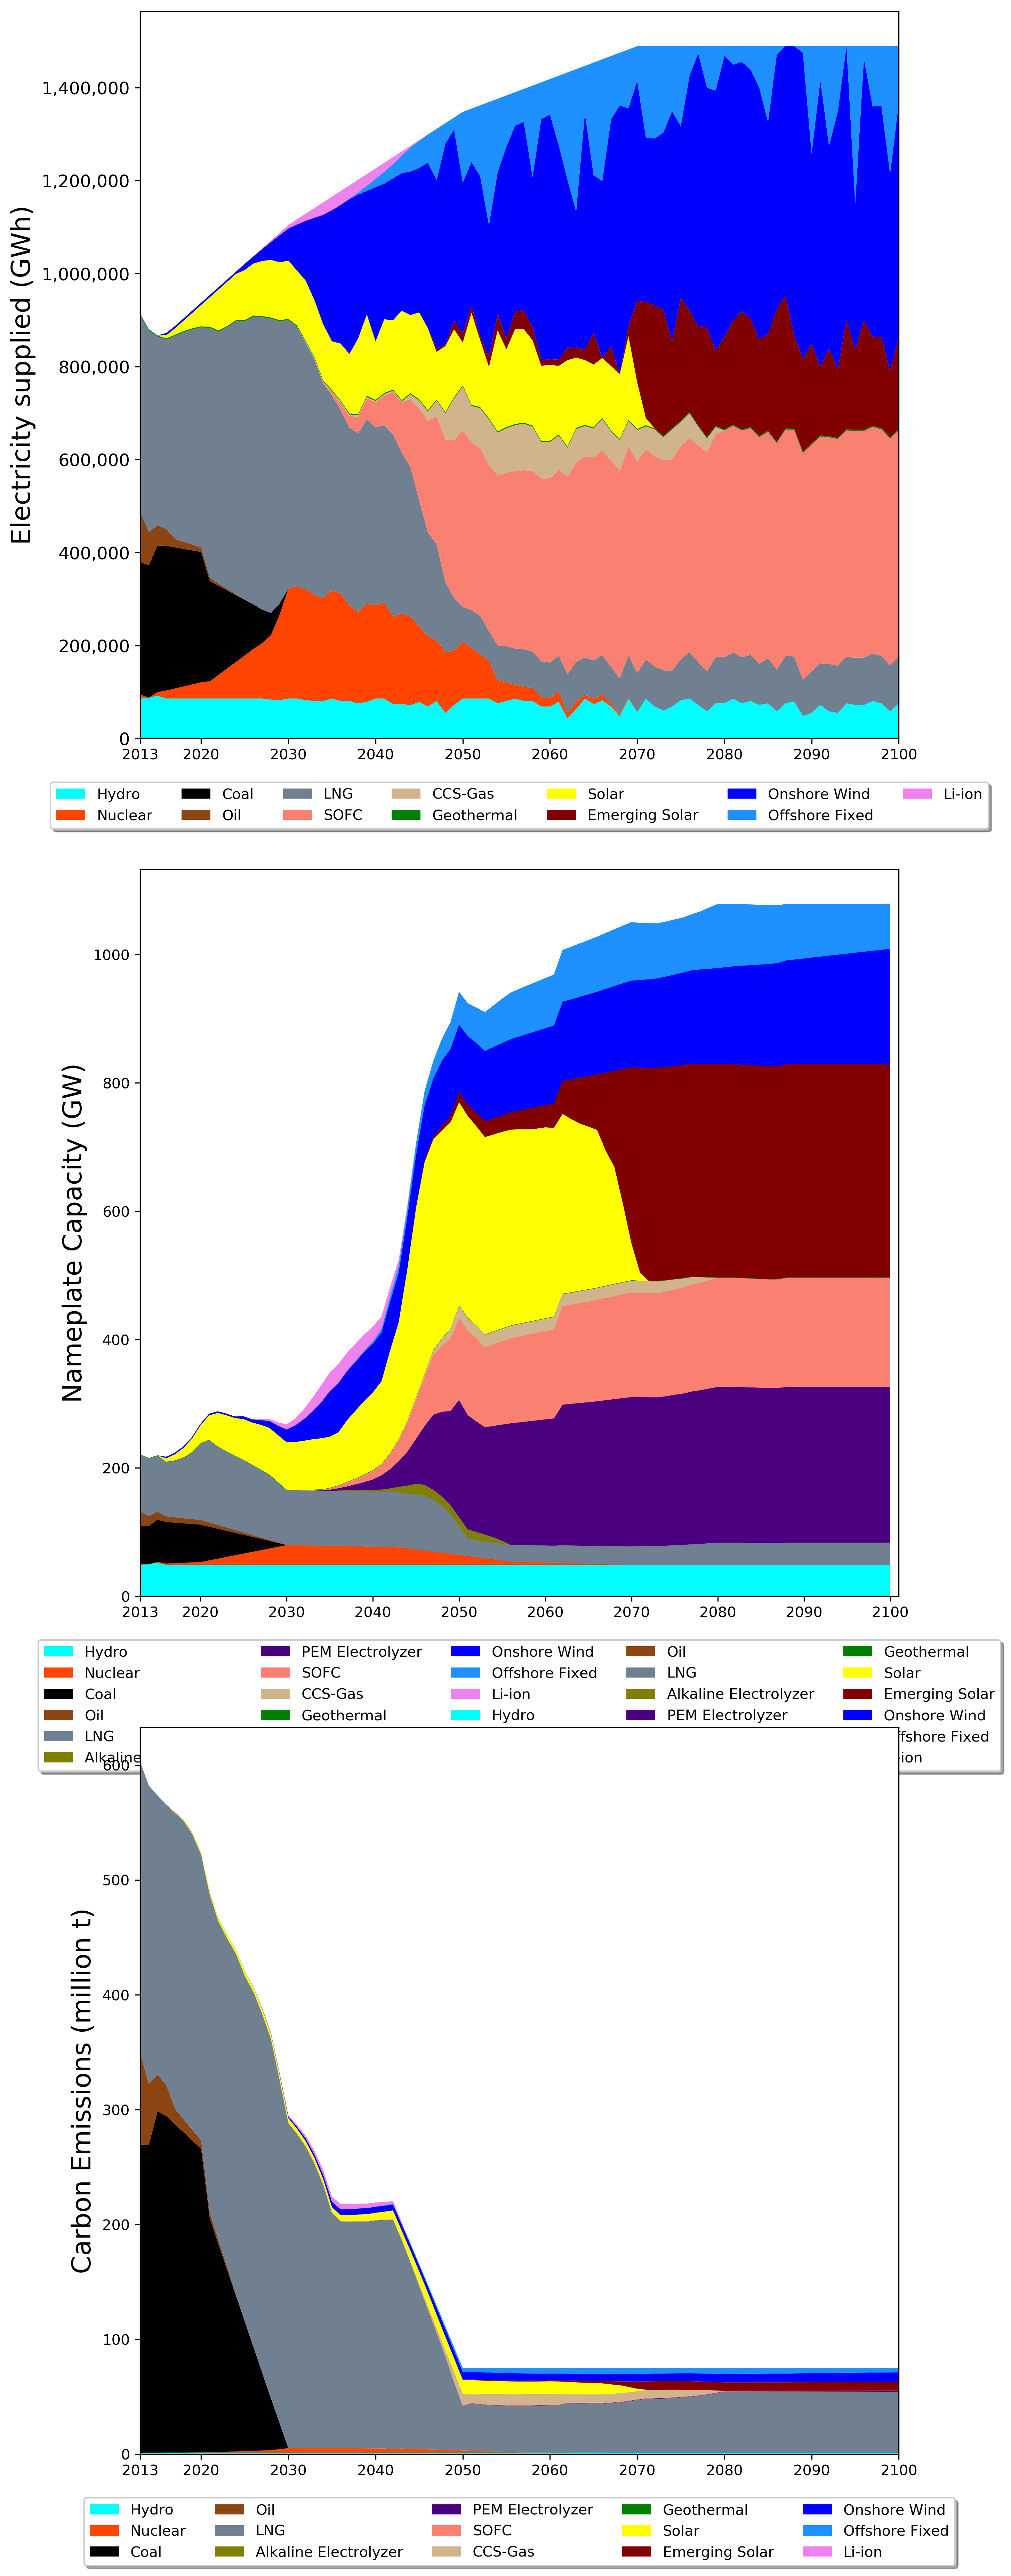
\includegraphics[scale=0.2]{figures/newtechs_nonuc}
\caption{Emerging technologies, no new nuclear.}
\end{figure}

\begin{figure}[h] 
\centering
\label{scen4}
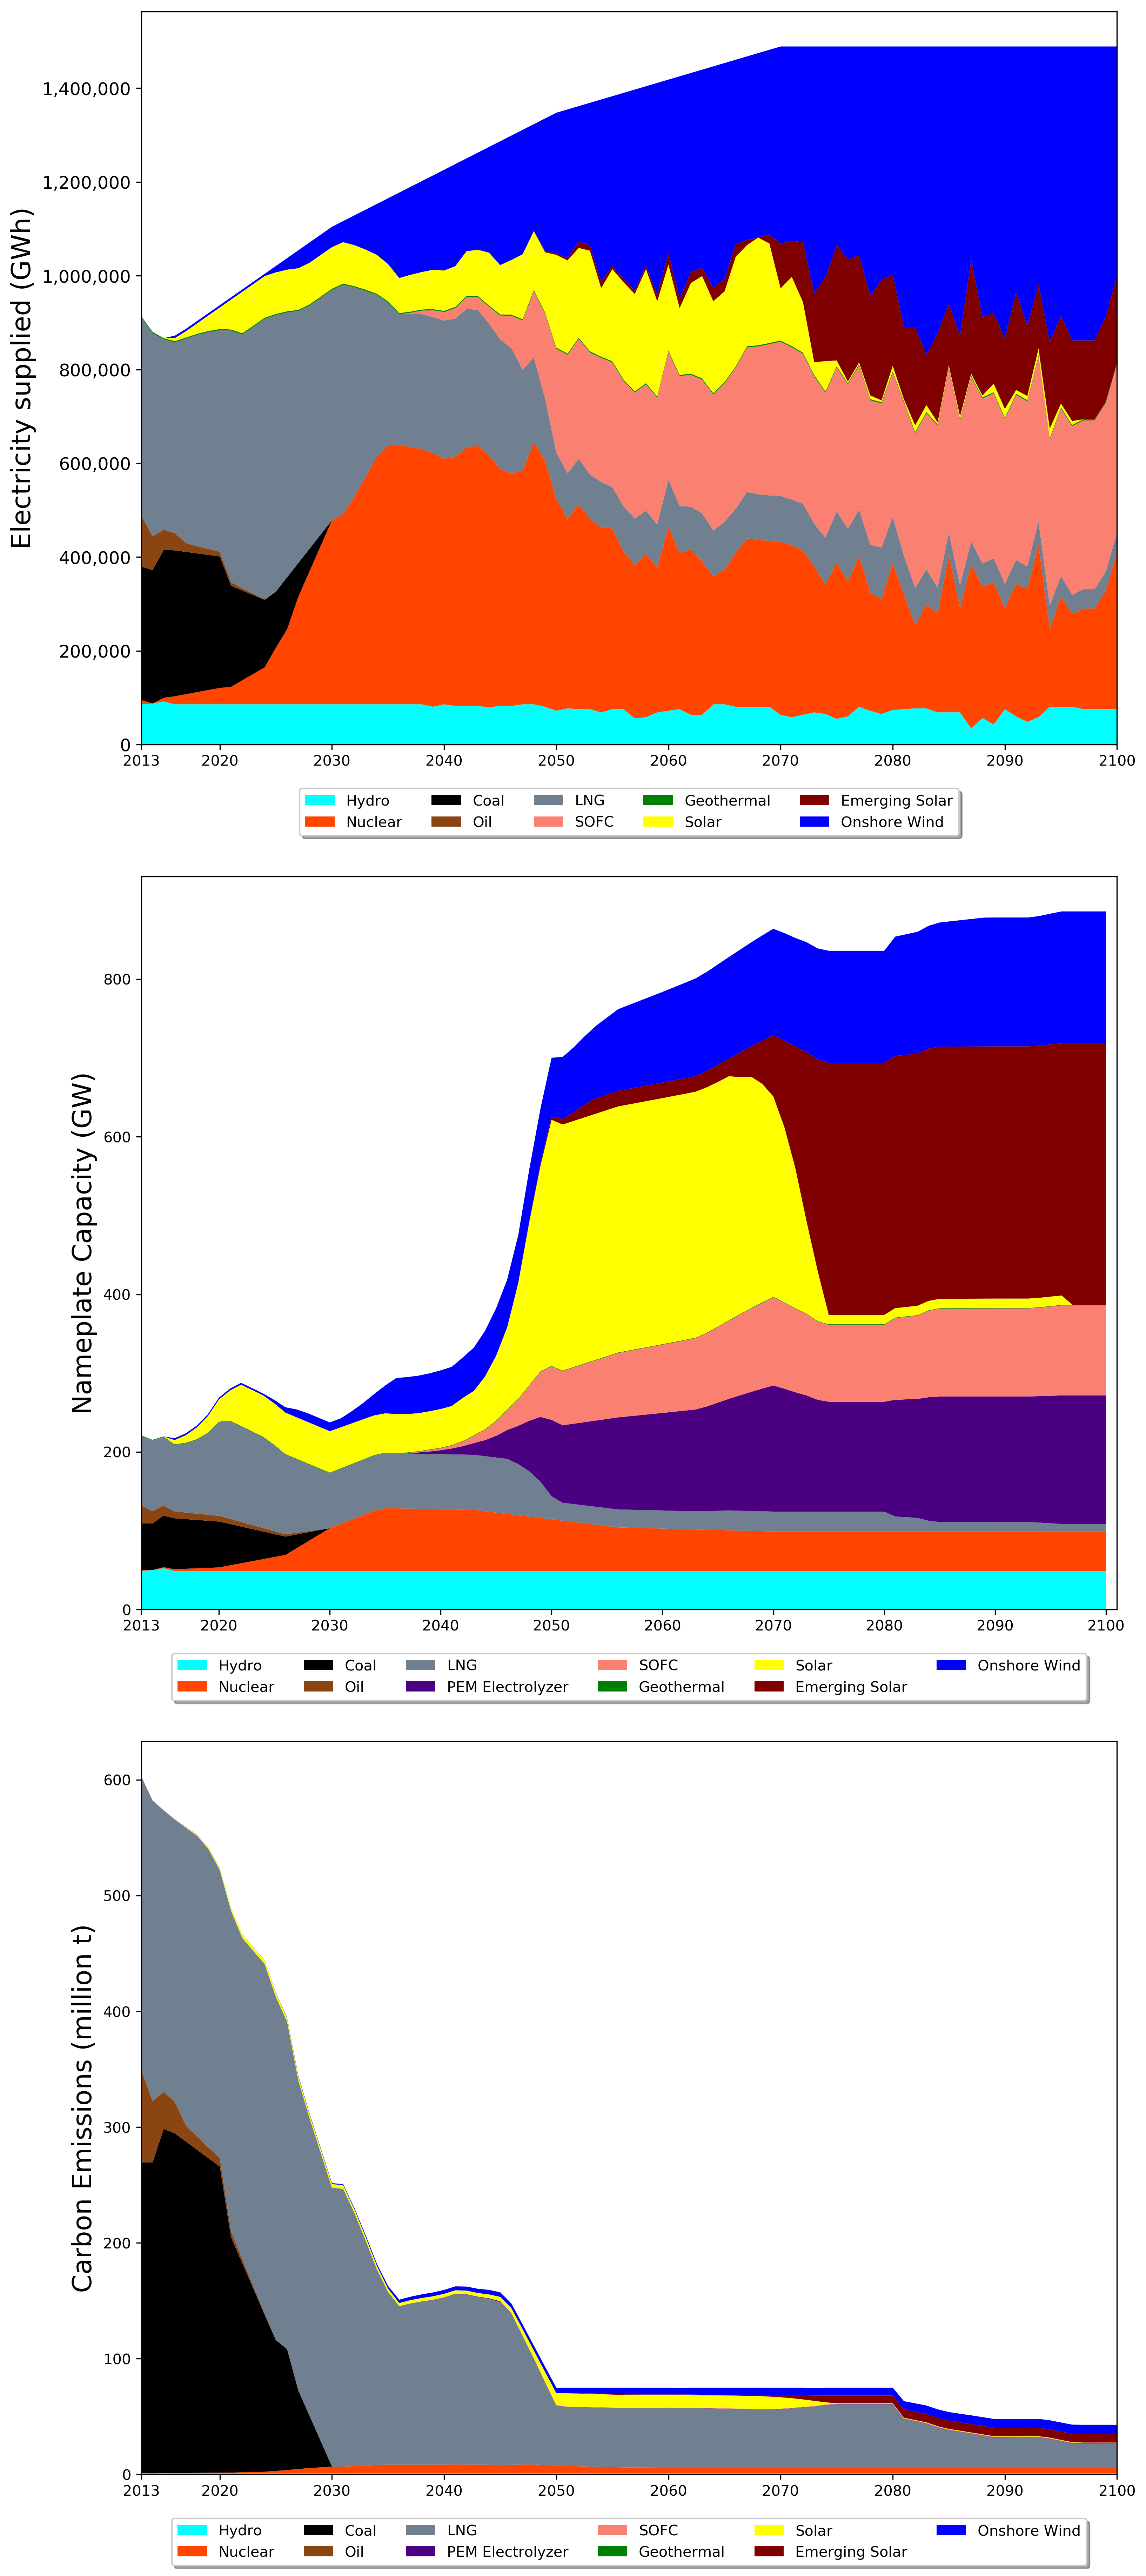
\includegraphics[scale=0.2]{figures/newtechs_nuc}
\caption{Emerging technologies, no new nuclear.}
\end{figure}

\subsection{Sensitivity analysis}